\documentclass[11pt]{article}

\usepackage[margin=1in]{geometry}
\usepackage{amsmath, amssymb}
\usepackage{graphicx}
\usepackage{booktabs}
\usepackage{xcolor}
\usepackage{listings}
\usepackage{hyperref}

\lstset{
  language=Python,
  basicstyle=\ttfamily\small,
  keywordstyle=\color{blue!70!black},
  commentstyle=\color{green!40!black},
  stringstyle=\color{red!60!black},
  frame=single,
  breaklines=true,
  showstringspaces=false,
  columns=fullflexible,
}

\title{MATH 7243 --- Lab 1: Exploratory Analysis}
\author{Wilson Glass}
\date{September 24, 2026}

\begin{document}
\maketitle

\section*{Setup and Data Cleaning}

The dataset is the truncated NYC AirBnB dataset (first 10{,}000 rows of the Kaggle
dataset). We keep only numerical columns and drop \texttt{host\_id}, which is an
identifier rather than a measurement. This leaves eight numerical features:
\texttt{latitude}, \texttt{longitude}, \texttt{price}, \texttt{minimum\_nights},
\texttt{number\_of\_reviews}, \texttt{reviews\_per\_month},
\texttt{calculated\_host\_listings\_count}, and \texttt{availability\_365}.

The raw data contains extreme outliers: the median price is about \$100 and the 99th
percentile is \$888, but the maximum is \$10{,}000; similarly \texttt{minimum\_nights}
reaches 1250. Following the approach in the Master notebook, we remove these with a
boolean mask, keeping listings with price below the 99th percentile and
\texttt{minimum\_nights} $\le 60$. This keeps 9{,}806 of the 9{,}999 rows. All results
below use this cleaned data.

\begin{lstlisting}
import numpy as np
import pandas as pd
from matplotlib import pyplot as plt

data = pd.read_csv("https://raw.githubusercontent.com/tipthederiver/Math-7243-2020/master/Datasets/NYCAirBnB/train.csv")

nums = data.select_dtypes(include=['int64','float64']).drop(columns=['host_id'])
z = (nums.price < nums.price.quantile(0.99)) & (nums.minimum_nights <= 60)
numsc = nums[z]
\end{lstlisting}

%-----------------------------------------------------------------------------
\section*{Problem 1: Histograms of the Numerical Features}

\begin{lstlisting}
f, axes = plt.subplots(2, 4, figsize=[20, 8])
axes = axes.reshape(-1)

for ax, name in zip(axes, list(numsc)):
    ax.hist(numsc[name].dropna(), bins=50, rwidth=.8)   # reviews_per_month has NaNs
    ax.set_title(name, fontsize=14)
for ax in axes[::4]:
    ax.set_ylabel("Count")

f.tight_layout()
plt.show()
\end{lstlisting}

\begin{figure}[h]
  \centering
  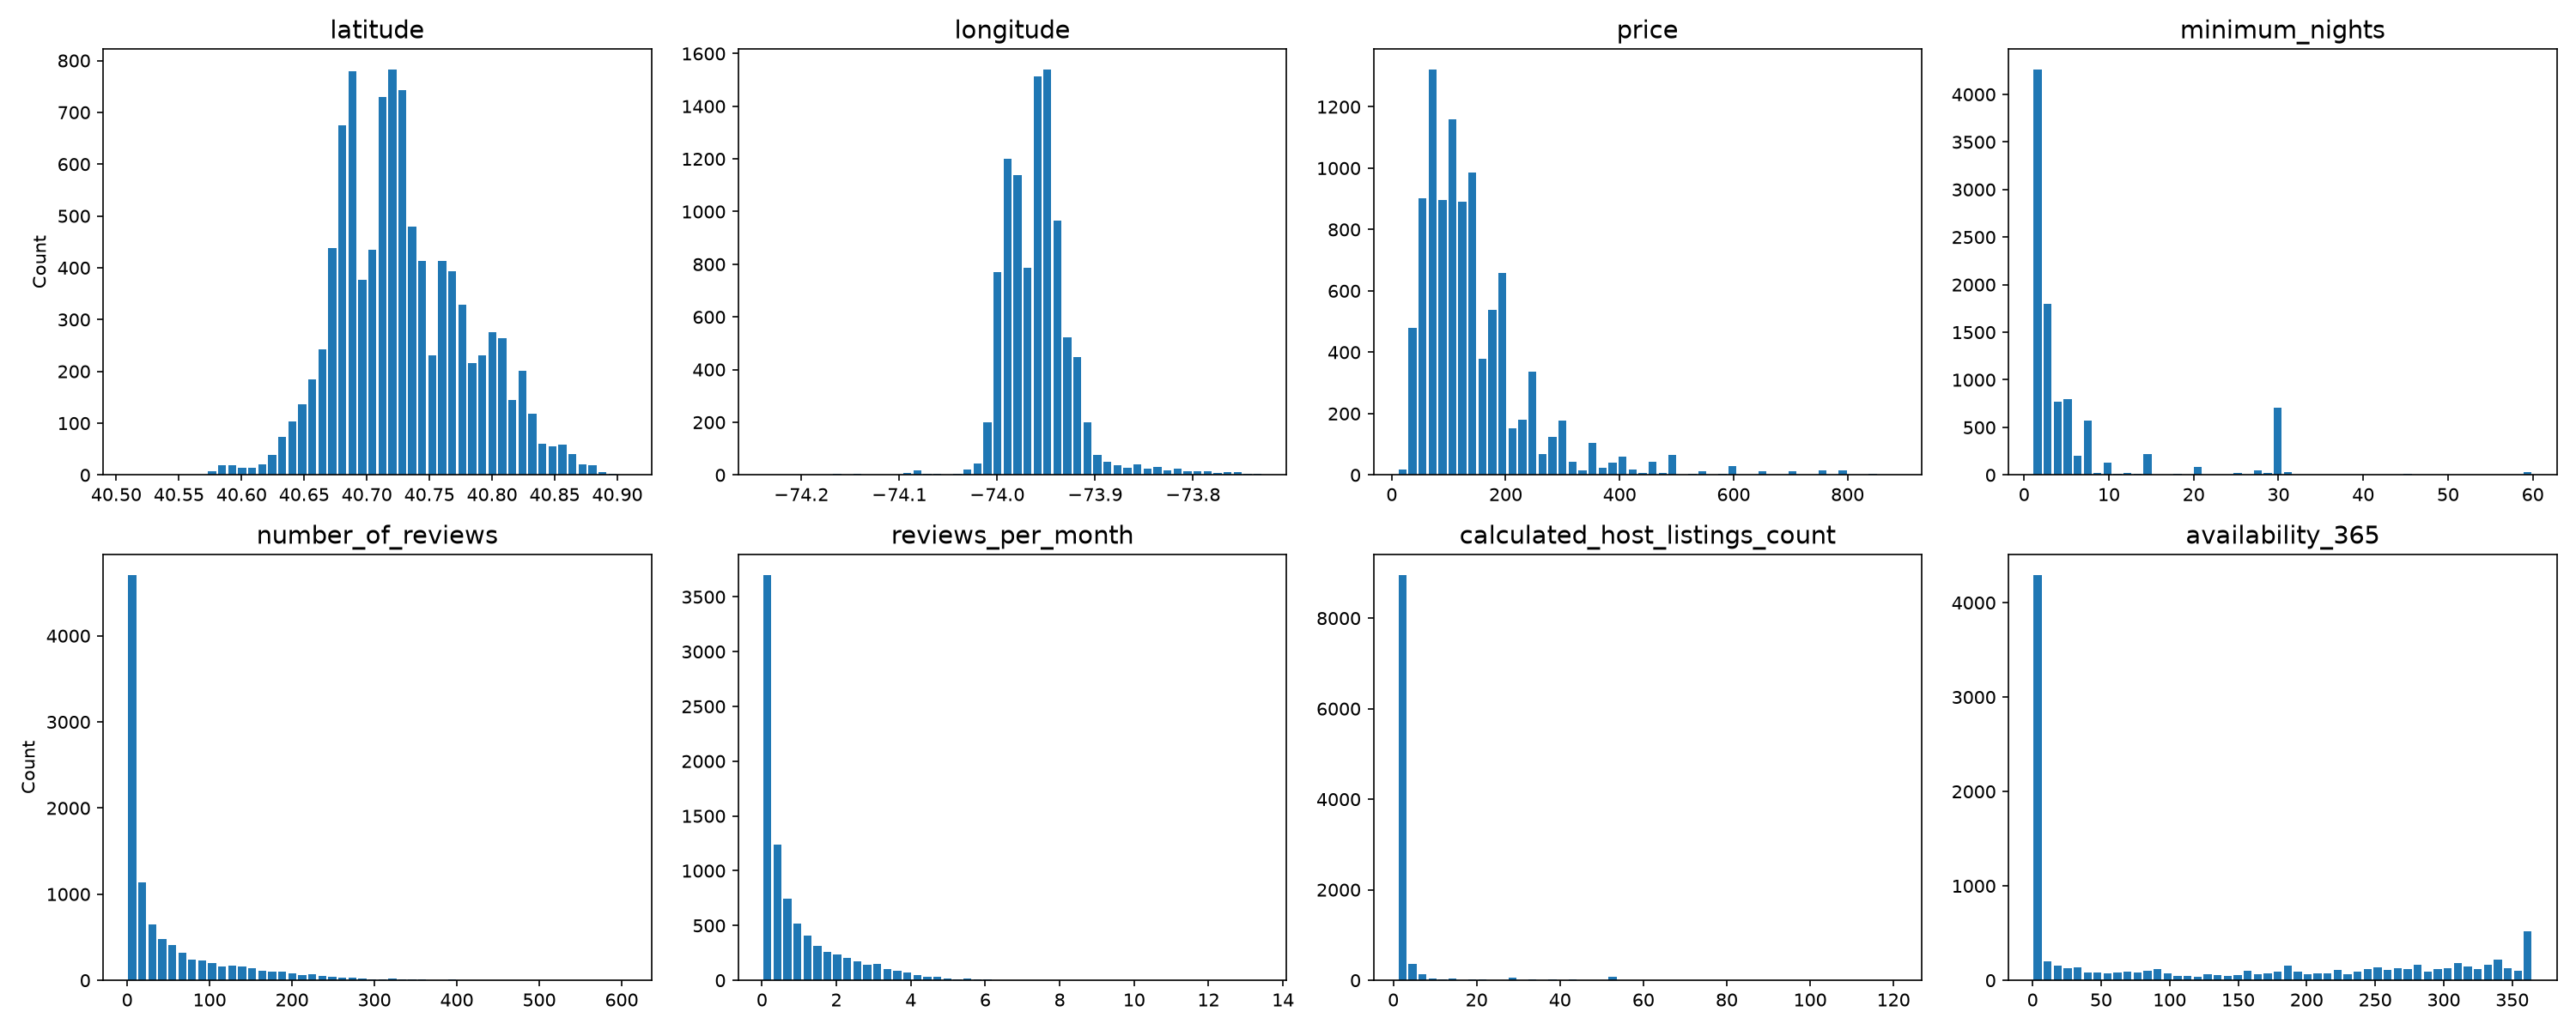
\includegraphics[width=\textwidth]{figures/histograms.png}
  \caption{Histograms of the numerical features (cleaned data).}
\end{figure}

Price is strongly right-skewed. \texttt{minimum\_nights} has a spike at 30
(monthly rentals), and \texttt{number\_of\_reviews}, \texttt{reviews\_per\_month}, and
\texttt{calculated\_host\_listings\_count} are concentrated near zero.

%-----------------------------------------------------------------------------
\section*{Problem 2: Scatter Plots of Price vs.\ Each Feature}

\begin{lstlisting}
features = [c for c in numsc.columns if c != "price"]  # to not include price vs price
f, axes = plt.subplots(2, 4, sharey=True, figsize=[20, 8])
axes = axes.reshape(-1)

for ax, name in zip(axes, features):
    ax.plot(numsc[name], numsc.price, 'o', markersize=2, alpha=.3)
    ax.set_title(name, fontsize=14)
for ax in axes[::4]:
    ax.set_ylabel("price")
for ax in axes[len(features):]:   # hide unused panel(s)
    ax.set_visible(False)

f.tight_layout()
plt.show()
\end{lstlisting}

\begin{figure}[h]
  \centering
  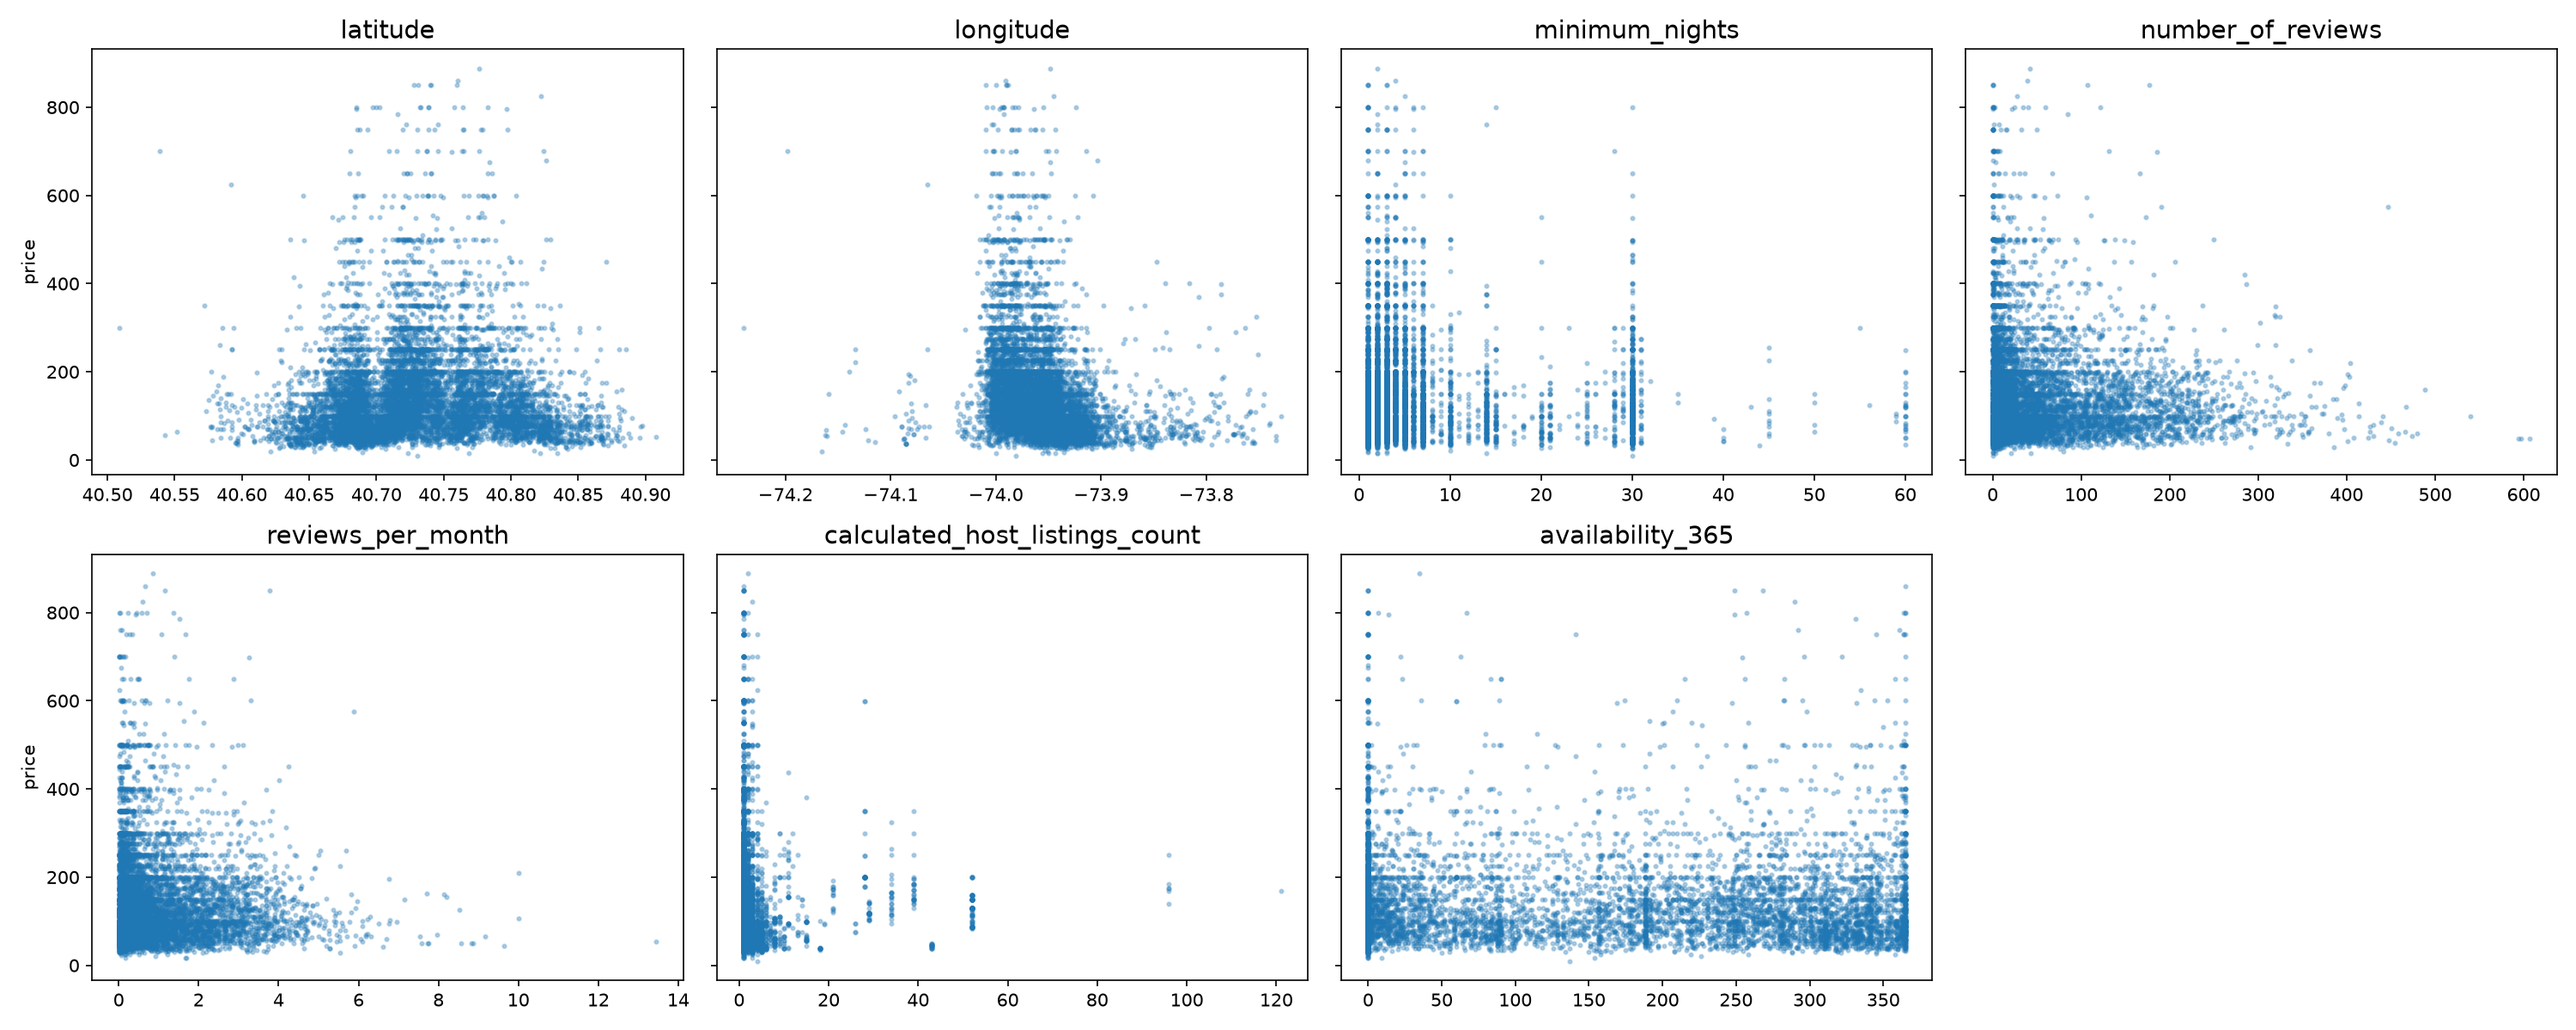
\includegraphics[width=\textwidth]{figures/scatter.png}
  \caption{Price against each numerical feature (cleaned data).}
\end{figure}

%-----------------------------------------------------------------------------
\clearpage
\section*{Problem 3: Correlation Matrix and Heatmap}

\begin{lstlisting}
import seaborn as sns

fig, ax = plt.subplots(figsize=(10, 8))
sns.heatmap(numsc.corr(), ax=ax, linewidth=.05, cmap="magma", annot=True, fmt=".2f")
plt.show()
numsc.corr()
\end{lstlisting}

\begin{figure}[h]
  \centering
  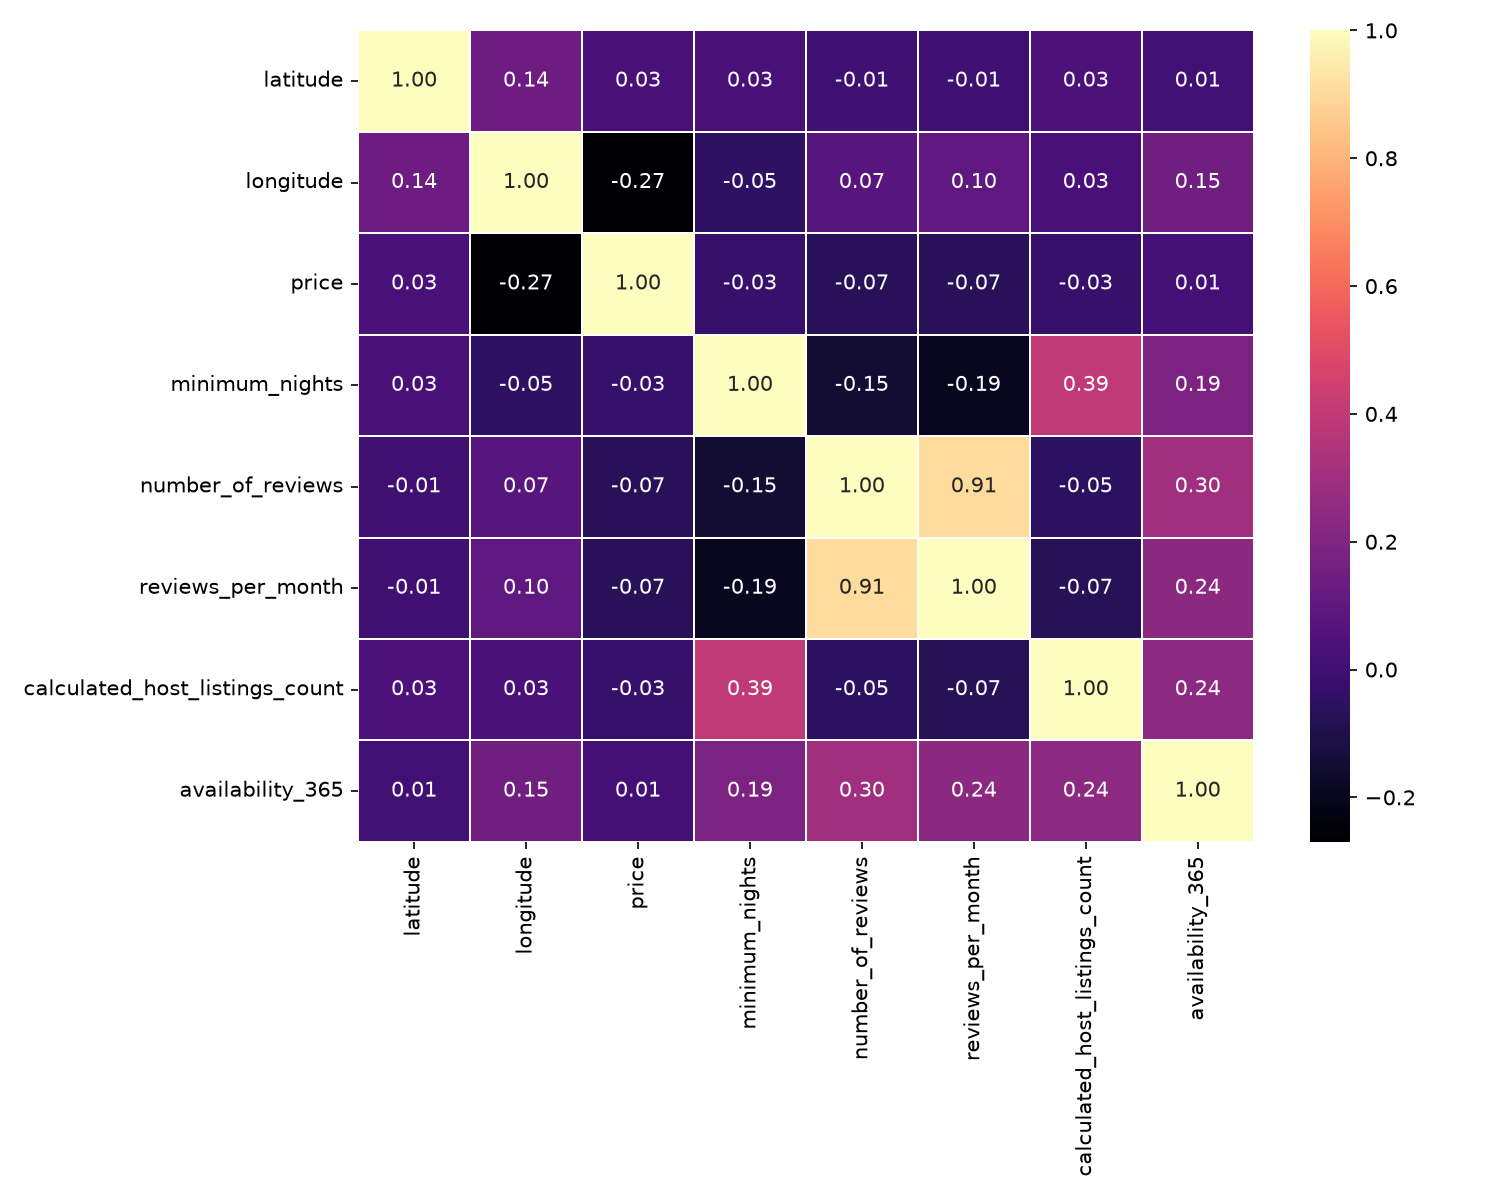
\includegraphics[width=0.8\textwidth]{figures/heatmap.png}
  \caption{Correlation heatmap of the numerical features (cleaned data).}
\end{figure}

%-----------------------------------------------------------------------------
\section*{Problem 4: Most Predictive Feature}

Using the correlation matrix from Problem 3, the correlation of each feature with
price is:

\begin{center}
\begin{tabular}{lr}
\toprule
Feature & Correlation with price \\
\midrule
\texttt{longitude}                      & $-0.270$ \\
\texttt{reviews\_per\_month}            & $-0.071$ \\
\texttt{number\_of\_reviews}            & $-0.068$ \\
\texttt{minimum\_nights}                & $-0.031$ \\
\texttt{latitude}                       & $0.029$ \\
\texttt{calculated\_host\_listings\_count} & $-0.027$ \\
\texttt{availability\_365}              & $0.009$ \\
\bottomrule
\end{tabular}
\end{center}

\textbf{Answer:} Longitude is the most predictive feature ($r \approx -0.27$).
Listings further west, in Manhattan, tend to cost more. All other features have
$|r| < 0.1$, so no single numerical feature predicts price strongly.

%-----------------------------------------------------------------------------
\section*{Problem 5: Linear Model and Predict Function}

We fit a linear model using all seven non-price numerical features. Let $X$ be the
$n \times 8$ design matrix whose first column is all ones (for the intercept) and whose
remaining columns are the features, and let $y$ be the vector of prices. Missing
values of \texttt{reviews\_per\_month} (listings with no reviews) are set to 0. The
parameters are found with the normal equation
\[
  w = (X^T X)^{-1} X^T y .
\]

\begin{lstlisting}
features = [c for c in numsc.columns if c != "price"]

X = numsc[features].fillna(0).to_numpy()     # NaN reviews_per_month -> 0
X = np.column_stack([np.ones(len(X)), X])    # column of 1s for the intercept w0
y = numsc.price.to_numpy()

w = np.linalg.inv(X.T @ X) @ X.T @ y         # normal equation: (X^T X)^-1 X^T y

def predict(X):
    return X @ w
\end{lstlisting}

The fitted parameters are:

\begin{center}
\begin{tabular}{llr}
\toprule
Parameter & Feature & Value \\
\midrule
$w_0$ & intercept                                & $-65836.24$ \\
$w_1$ & \texttt{latitude}                        & $136.49$ \\
$w_2$ & \texttt{longitude}                       & $-817.01$ \\
$w_3$ & \texttt{minimum\_nights}                 & $-0.83$ \\
$w_4$ & \texttt{number\_of\_reviews}             & $-0.07$ \\
$w_5$ & \texttt{reviews\_per\_month}             & $-4.28$ \\
$w_6$ & \texttt{calculated\_host\_listings\_count} & $-0.33$ \\
$w_7$ & \texttt{availability\_365}               & $0.07$ \\
\bottomrule
\end{tabular}
\end{center}

\textbf{Predict function:}
\begin{align*}
  \hat{y} = -65836.24 &+ 136.49\,x_1 - 817.01\,x_2 - 0.83\,x_3 - 0.07\,x_4 \\
                      &- 4.28\,x_5 - 0.33\,x_6 + 0.07\,x_7,
\end{align*}
where $\hat{y}$ is the predicted price and $x_1, \dots, x_7$ are latitude, longitude,
minimum nights, number of reviews, reviews per month, calculated host listings count,
and availability (days per year), respectively.

The large intercept offsets the large magnitudes of latitude ($\approx 40.7$) and
longitude ($\approx -74$); it has no direct interpretation on its own.

%-----------------------------------------------------------------------------
\section*{Problem 6: RSS Cost}

The residual sum of squares is
\[
  \text{RSS} = \sum_{i=1}^{n} (y_i - \hat{y}_i)^2 = (y - Xw)^T (y - Xw).
\]

\begin{lstlisting}
rss = np.sum((y - predict(X)) ** 2)
print(f"RSS = {rss:,.2f}")
\end{lstlisting}

\textbf{Answer:} $\text{RSS} = 92{,}454{,}879.10$.

For context, over $n = 9{,}806$ listings this corresponds to a root-mean-square error
of $\sqrt{\text{RSS}/n} \approx \$97$, and $R^2 = 1 - \text{RSS}/\text{TSS} \approx 0.09$.
The numerical features explain only about 9\% of the variation in price, so the model
is a weak fit. This is consistent with the low correlations in Problem 3: much of what
determines an AirBnB's price (room type, borough) is contained in the categorical
features, which this model does not use.

\end{document}
